% Explain the genral stucture of the debugger
The acutal debugger called \emph{Embedded Rust Debugger}(the code for the debugger can be found in the git repository \cite{erd}) consists mainly of two main threads called the \emph{main thead} and the \emph{debug thread}.
The \emph{main thead} is the thread that handels the input from the user from the console or trough \gls{dap} and the \emph{debug thread} handles the reading of \gls{DWARF} information and connection to the \gls{debugee}.
There is also another thread in the debugger called \emph{input thread} that is only activated if the user is using the console, its jobb is to read the input and send it to the \emph{main thread}.


% Explain the first state where the debugger is not attach to the debugee
The debug thread has two main state that it changes between, the first state is when it is not attached to any \gls{debugee} and is called DebugHandler.
The second state is when it is attach to the \gls{debugee} which means that this state is where debugging can happen, it is called Debugger.
Going back to the fist state, its purpose is to await instructions to attach to the \gls{debugee} and to receive configuration required for that to happen.
These configurations that the debugger requires is a path to the elf file, a path to the work directory of the code that should be debugged and lastly the type of chip.
When all these are configure the attach command can be used to attach to the micro controller, all the other commands that require that the chip is attach can also be used to attach.


% Explain the second state where the debugger is attach to the debugee.
The debugger uses the library \emph{probe-rs} \cite{probe} to attach to the micro controller and to interact with it.
Thus a lot of useful debugging features like stopping, continuing and setting hardware breakpoints is already given by the \emph{probe-rs} library.
The other features supported by the debugger uses the library \emph{rust-debug} together with the \emph{probe-rs} library.
But the two library are separate so they never interact with each other, the figure \ref{fig:debugger} show how all of these parts interact.
The \emph{rust-debug} library as mention above and seen in the figure \ref{fig:debugger} is a library for retrieving information from the \emph{DWRAF} sections in the \gls{elf} file.
To get some of the information from the library values in the \glspl{debugee} memory and/or registers are needed.
Thus when the \emph{rust-debug} library gives a response to a requires that it needs some specific value the \emph{Debugger} \emph{Rust} struct can use \emph{probe-rs} to read those values.
Then those values can be sent in as a argument or the \emph{rust-debug} library.
This repeats until the \emph{rust-debug} library returns the requested value or an error.


\begin{figure}[h]
	\centering
	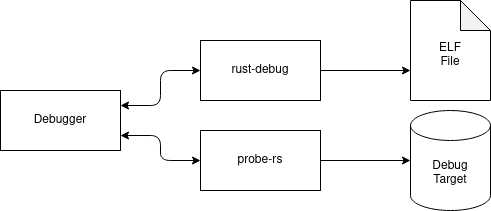
\includegraphics[width=1.0\textwidth]{debugger.png}
	\caption{A diagram showing the relations between the debugger, the \emph{ELF} file, the \gls{debugee} and the two libraries \emph{rust-debug} and \emph{probe-rs}.}
	\label{fig:debugger}
\end{figure}


% How the debugger handles request and events simultaneously.
To simultaneously handle incoming request from the user and events that happens in the \gls{debugee}, the debugger polls the channel for incoming request and the state of the debugger.
To reduce the amount of polling of the state of the \gls{debugee} the debugger has a boolean that keeps track of the state of the \gls{debugee}.
This boolean is to track if the \gls{debugee} is running or is stopped.
And because events can only occur if the \gls{debugee} is running the polling only needs to be done when it thinks the \gls{debugee} is running.
Thus this is how the debugger can handle request from the user and near simultaneously handle events that happen in the \gls{debugee}.


% How it handles request for stackframes and variables.
To improve of the performance of the debugger the debugger stores the value of the stack frames every time they are calculated.
This allows for fast repetitive look up of stack frame information and variables.
The stored stack frame values are only stored when the \gls{debugee} is stopped and are removed when the \gls{debugee} starts.
Thus the wrong values will never be shown to the user.
Also another feature of the debugger is that if the value of a variable is request the debugger will restive all the stack frames instead and then search for the requested variable.
This simplifies the implementation a lot and will also make the debugger faster when repeated request are made.

